\chapter{Razvrščanje besedil}

V prejšnjih dveh poglavjih so predlagane tehnike razvrščanja
predpostavljale, da lahko razdaljo, ali pa podobnost med primeri
enostavno izračunamo. Vsi naši primeri so bili opisani atributno in
razdalja je bila lepo določena z, na primer, razdaljo v evklidskem
prostoru. Podatke smo morali predobdelati in vsakega od
atributov normalizirati, drugih, bolj kompleksnih priprav podatkov pa
postopki razvrščanja niso zahtevali.

Drugače je s tekstovnimi dokumenti, ali besedili. Vzemimo na
primer, da moramo v skupine urediti naslednje tri novice:

{\small
\begin{quotation}
Na odru ljubljanske Drame se drevi ustavlja prva slovenska godba na pihala, ki že več kot 15 let preigrava skoraj izključno ulični džez New Orleansa. Cerkljanski Kar Češ Brass Band, ki neworleanški džez interpretira na svojevrsten in svež način, so v gledališče povabili v sklopu cikla Drama Akustika.
\end{quotation}

\begin{quotation}
Tretji oktobrski konec tedna na Ravnah na Koroškem zdaj že tradicionalno poteka Festival slovenskega jazza, katerega spremljajoči dogodki se na Koroškem vrstijo že od septembra. Tridnevni festivalski vrhunec je v Kulturnem centru Ravne odprl Big Band RTV Slovenija z vsestranskim glasbenikom Boštjanom Gombačem.
\end{quotation}

\begin{quotation}
Murskosoboški policisti so 33-letniku z območja Murske Sobote zasegli
posušeno konopljo, sadike in gotovino, za katero sumijo, da jo je
dobil s preprodajo. Pri tem so v hiši osumljenega odkrili poseben
prostor za gojenje konoplje pod umetno svetlobo. V tem prostoru so
našli in zasegli tudi 20 sadik konoplje, visokih do 90 centimetrov, in
dober kilogram posušene oz. delno posušene konoplje.
\end{quotation}
}

Nam, ljudem, je ta razvrstitev enostavna. Zadnja, tretja novica, sodi
v črno kroniko, prvi dve pa med kulturne novice.

Programsko razvrščanje novic s tehnikami iz prejšnjega poglavja pa ni
trivialno. Očitno bomo morali določiti nove mere, ki nam bodo pomagale
oceniti, kako različna so si med sabo besedila. Pristopi k razvrščanju
dokumentov, ki jih predlagamo v tem poglavju, temeljijo na
preoblikovanju besedil v atributno obliko, kjer je moč take mere
določiti, da bi nato za razvrščanje uporabili tehnike, kot sta
hierarhično razvrščanje v skupine in metodo voditeljev, ki jih že
poznamo.

\section{Elementi predstavitve besedilnih dokumentov}

\subsection{$k$-terke znakov}

``Murskosoboški'' lahko predstavimo z dvojkami ``mu'', ``ur'', ``rs'',
..., torej s pari znakov, ki si sledijo v zaporedju. Za vsak par lahko
izračunamo frekvenco pojavitve v besedilu oziroma relativno frekvenco,
ki je enaka ocenjeni verjetnosti pojavitve $k$-terke. 

Število $k$-terk je veliko že za pare ($n=2$), za večje vrednosti $k$
pa jih je mnogo ali ogromno. V praksi se uporabljajo $k$-terke do
$n=5$. Zanimivo pa je, da je že porazdelitev dvojk lahko
karakteristična za posamezne jezike in lahko na podlagi teh
razpoznamo, v katerem jeziku je napisano določeno
besedilo\footnote{Glej
  \url{www.lingua-systems.com/language-identifier/lid-library/identify-language.html}}. Za
bolj zahtevne naloge je potrebno seveda uporabiti daljše $k$-terke.

Ta predstavitev je načelno enostavna, a jo precej oteži uporaba
posebnih znakov, ki jih moramo ali upoštevati ali pa primerno
predobdelati besedilo.

\subsection{Besede}

Dokumente lahko predstavimo z vrečo besed \angl{bag of words}, to je s
skupino besed in številom njihovih pojavitev v dokumentu. Pri tem
lahko besedilo najprej predobdelamo:
\begin{itemize}
\item odstranimo manj pomembne besede \angl{stop-words}, ki so za
  slovenščino na primer ``in'', ``ali'', ``ter'', ipd.
\item vse besede nadomestimo z njihovimi koreni ali pa lemami. V
  računalništvu je lematizacija algoritmični postopek določevanja leme
  določeni besedi. Postopek ni enostaven in je tipično odvisen od
  jezika, v katerem je zapisano besedilo. Za angleščino je na primer
  znan Porterjev iskalnik korenov besed \angl{Porter stemmer}, ki je
  sestavljen iz ročno izdelanih pravil\footnote{Implementacija
    Porterjevega korenjenja v različnih programskih jezikih je
    dostopna na \url{http://tartarus.org/martin/PorterStemmer}}.
\end{itemize}

Predstavitev z vrečo besed zanemarja dejstvo, da je pomen besed
mnogokrat odvisen od konteksta. Ista beseda ima lahko različne pomene,
ali pa imajo isti pomen lahko različne besede. Prav tako nam taka
predstavitev ne bo mogla razrešiti problema podpomenk in drugačnih
povezav med različnimi izrazi.

Število pojavitev besed v dokumentu je seveda odvisno od dolžine
dokumenta. Da ta vpliv izničimo, namesto števila pojavitev besed
uporabljamo relativno frekvenco, to je verjetnost, da bi pri
naključnem izboru besede iz dokumenta izbrali določeno besedo.

\iffalse
Primer predobdelave besedila v programskem jeziku Python s knjižnico
iz paketa Orange je podan spodaj. Koda odstrani nepomembne besede,
ustvari seznam besed ter besedam iz tega seznama poišče leme.

\begin{python}
import orngText

def preprocess(text):
    pp = orngText.Preprocess(language='en')
    text.lower()
    text = pp.removeStopwords(text)
    tokens = pp.tokenize(text)
    lemmas = pp.lemmatize(tokens)
    
    print "Text:", text
    print "Tokens:", " ".join(tokens)
    print "Lemmas:", " ".join(lemmas)
    return lemmas

preprocess("The main point of writing a text is to convey " +
           "ideas, information, or knowledge to the reader.")
preprocess("He ensnared in an insider trading investigation " +
           "and a former director is expected to " +
           "surrender to authorities.")
\end{python}
\fi

\subsection{Fraze}

Fraze so lahko $k$-terke besed, ki se v besedilu nahajajo neposredno
druga ob drugi ali pa v bližnji okolici. Okolico lahko določa, na
primer, okno zaporedja petih besed. Težava pri tej predstavitvi je, da
je lahko možnih kombinacij že za pare besed ogromno. Pred leti je
Google objavil svojo zbirko fraz~\footnote{Glej
  \url{http://googleresearch.blogspot.com/2006/08/all-our-n-gram-are-belong-to-you.html}.},
ki jih je odkril iz besedilnih dokumentov. Vsebovala je na primer
314.843.401 pare besed, 977.069.902 trojk, 1,313,818,354 četvorčkov in
1,176,470,663 fraz s petimi besedami.

Uporaba fraz je smiselna ob souporabi fraznega korpusa, to je, baze že
znanih oziroma izbranih fraz za določeno problemsko
področje. Predstavitev z vrečo besed je načelno ustrezno moč dopolniti
s frazami iz besedila, tako da vsaka fraza tvori nov atribut.

\subsection{Besedne vrste}

Koristi nam lahko tudi prepoznavanje besednih vrst
\angl{part-of-speech}, kot so imena ljudi, krajev, organizacij. Za
prepoznavanje besednih vrst bomo morali uporabiti algoritme, ki znajo
besedilo analizirati veliko globlje in pri tem uporabljajo lingvistično
znanje ali pa vnaprej pripravljeni korpus. Seveda bo taka analiza tudi
odvisna od uporabljenega jezika. Pri katerih besedah v spodnjem
besedilu bi določitev besednih vrst lahko bila koristna pri analizi?

\begin{python}
We walk down the dirty old street.
The mailbox stood on the walk.
We heard cries echoing in the night.
The babied cries all night.
\end{python}

\subsection{Taksonomije}

V splošnem se taksonomija nanaša na stopenjsko razvrstitev
stvari. Pomaga nam pri ugotavljanju povezanosti med stvarmi, pri bolj
podrobnih taksonomijah pa iz njih zvemo še za
vrsto relacije. Primer take taksonomije za angleške besede je
WordNet~\footnote{WordNet je prosto dostopen na naslovu
  \url{http://wordnetweb.princeton.edu}.}. Odlična vizualizacija
povezav med besedami, kjer je prikazan tudi pomen povezav, je dostopna
na spletni strani Visuwords \footnote{\url{http://www.visuwords.com/}}
(slika \ref{f-visuwords}). Enostavnejša oblika zapisa take taksonomije je
slovar sopomenk ali tezaver \footnote{Glej
  npr. \url{http://www.tezaver.si/}.}.

\begin{figure}[htbp]
\begin{center}
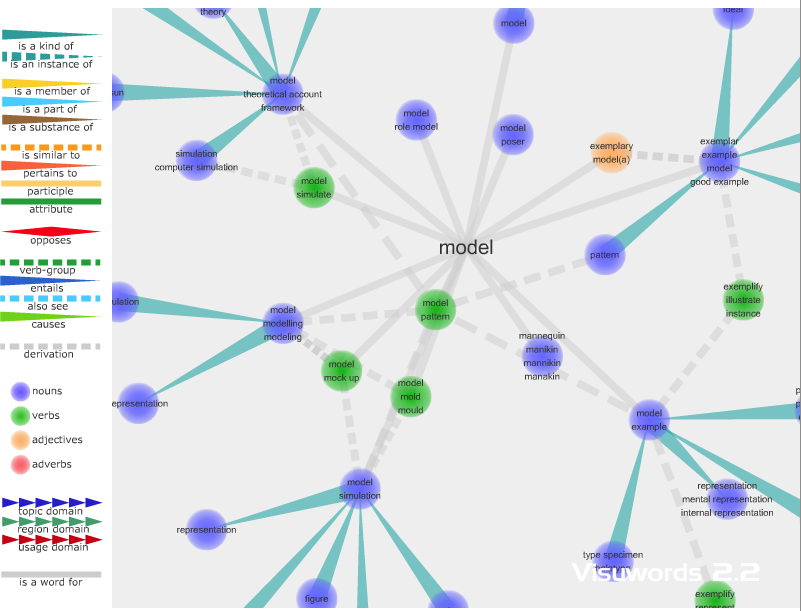
\includegraphics[width=15cm]{slike/visuwords.png}
\caption{Del taksonomije okoli angleške besede ``model'', kot jo
  prikaže spletna aplikacija Visuwords.}
\label{f-visuwords}
\end{center}
\end{figure}


\subsection{Slovnična analiza}

K računalniškem razumevanju besedila bi seveda zelo pripomogla
slovnična analiza. Uporabe tovrstnega globljega razumevanja besedila
pri razvrščanju dokumentov je predmet velikega števila trenutnih
raziskav. Prav možno je, da bodo v prihodnosti te, bolj kompleksne
jezikovne tehnologije nadomestile plitvejše, statistične tehnike ki
uporabljajo štetje parov črk ali preštevanje besed. A je prav
enostavnost slednjih in točnost, ki jo omogočajo že ti izjemno
preprosti pristopi ena od ovir za prevlado bolj kompleksnih
tehnologij.

\subsection{Uporaba pripadajočih oznak}

Mnogo dokumentov je danes označenih. Naj bodo to spletne strani
(npr. \url{del.icio.us}), dokumenti v raznih zbirkah, zapisi v
programu EverNotes, seznami bibliografskih enot v skladiščih povzetkov
CiteULike\footnote{\url{www.citeulike.org}} ali
PubMed\footnote{\url{http://www.ncbi.nlm.nih.gov/pubmed/}}. Oznake so
lahko bile prosto izbrane, ali pa vzete iz posebej za to določenega
slovarja ali pa ontologije. Dokumente lahko označujejo vsi, ki imajo
do njih dostop, ali pa samo pooblaščeni uporabniki ali kuratorji. V
vsakem primeru nam oznake lahko služijo kot osnova za predstavitev
vsebine dokumentov in zamenjujejo ali pa dopolnjujejo elemente, kot
smo jih predstavili zgoraj.

\begin{figure}[htbp]
\begin{center}
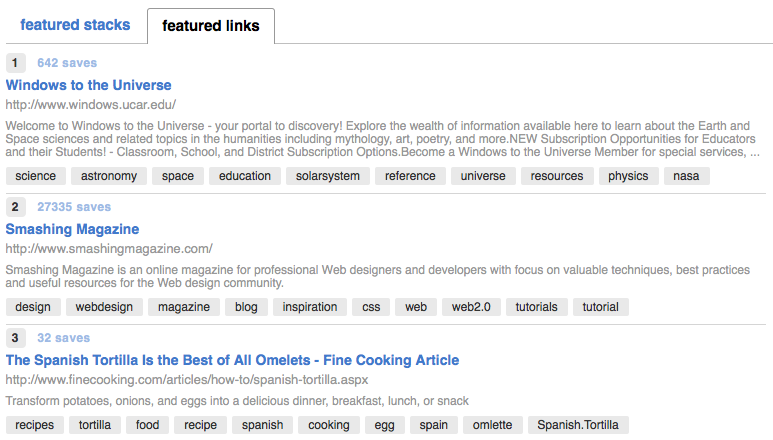
\includegraphics[width=15cm]{slike/delicious.png}
\caption{Oznake spletnih strani, kot so jih uporabniki določili v
  družabnem okolju del.icio.us.}
\label{f-delicious}
\end{center}
\end{figure}


\section{Ocenjevanje podobnosti med dokumenti}

V tem besedilu se bomo omejili na najpreprostejšo obliko predstavitve,
kjer besedilni dokument predstavimo z vektorjem enot in njihovo
frekvenco ali relativno frekvenco. Nestrukturiran dokument torej
predstavimo z atributnim jezikom. Ker je atributov lahko zelo veliko,
in ker vsi dokumenti nimajo nujno določene vse atribute, je matrika z
dokumenti v vrsticah in vrednosti atributov v kolonah zelo
prazna. Namesto te predstavitve lahko zato uporabimo slovar, z
elementi kot ključi in njihovimi frekvencami kot vrednostmi.

\subsection{Transformacija tf-idf}

Pogostost elementa (besede, terke) v dokumentu je enostavno število
pojavitev tega elementa v dokumentu. Če bi uporabljali to število, bi
prihajalo do večjih razlik med daljšimi in krajšimi dokumenti. Zato
pogostost pojavitve normaliziramo in namesto njih uporabljamo
relativne frekvence, oziroma iz dokumenta ocenimo verjetnosti
pojavitve določenega elementa. To označimo z $\mathrm{tf}(t,d)$
\angl{term frequency}.

Načelno imamo raje elemente, ki se pojavljajo v manj dokumentih in so
zaradi tega bolj specifični. Na osnovi elementov, ki se pojavijo v
večini dokumentov, bi te zelo težko razlikovali. Zato uvedemo pojem
inverzne frekvence v dokumentih \angl{inverse document frequency}, ki
jo uporabljamo kot splošno mero za pomembnost določenega elementa:
$$\mathrm{idf}(t) =  \log \frac{|D|}{|\{d: t \in d\}|}$$
kjer je $|D|$ število dokumentov v množici dokumentov $D$ in $|\{d : t
\in d\}|$ število dokumentov, ki vsebujejo element $t$ (torej, kjer je
$\mathrm{tf}(t,d) \neq 0$). Če elementa ni v korpusu, bi zgornje
vodilo k deljenju z 0. Zato lahko zgornji izraz prilagodimo in
zapišemo $1 + |\{d : t \in d\}|$.

Utež elementa $t$ v danem dokumentu $d$ je potem zmnožek njegove
frekvence v tem dokumentu in splošne pomembnosti tega elementa:
$$\mathrm{tf\mbox{-}idf}(t,d) = \mathrm{tf}(t,d) \times \mathrm{idf}(t)$$

\subsection{Kosinusna podobnost}

Čeprav bi za merjenje razdalj med vektorji, ki predstavljajo
dokumente, lahko uporabljali tudi Evklidsko razdaljo (glej prejšnje
poglavje), se ta na področju obravnave besedilnih dokumentov ne
uporablja. Razlog je preprost. Imejmo dva vektorja, $X$ in $Y$ in
predpostavimo, da sta zelo različnih velikosti, a da kažeta v isto
smer. Evklidska razdalja med njima je lahko večja kot med vektorjema,
ki bi bila kratka, a kazala v popolnoma različne smeri. Na področju
besedilnih dokumentov smer vektorja ustreza specifičnemu profilu
dokumenta v smislu vsebovanosti posameznih elementov. Pomembna je
smer, kamor kaže vektor, in manj (ali pa čisto nič) njegova
dolžina. Razliko med smerjo dveh vektorjev lahko merimo s kotom med
vektorji, ta pa je proporcionalna kosinusu kotov. Za dva vektorja
$\mathbf{a}$ in $\mathbf{b}$ velja:
$$\mathbf{a}\cdot\mathbf{b}
=\left\|\mathbf{a}\right\|\left\|\mathbf{b}\right\|\cos\theta$$
Podobnost med primeroma $X$ in $Y$ lahko zato zapišemo kot:
$$\text{sim}(X,Y) = \cos(\theta) = {X \cdot Y \over \|X\|\ \|Y\|}
= \frac{ \sum_{i=1}^{m}{X_i \times Y_i} }{
  \sqrt{\sum_{i=1}^{m}{(X_i)^2}} \times \sqrt{\sum_{i=1}^{m}{(Y_i)^2}}
}$$

\subsection{Podobnost po Jaccardu}

Kadar imamo opraviti z oznakami (torej, ne z besedami iz besedila, pri
katerih poleg vsebnosti opazujemo tudi število pojavitev) je poleg
kosinusne razdalje smiselno opazovati tudi podobnost po Jaccardu:
%
$$J(X,Y) = {{|X \cap Y|}\over{|X \cup Y|}}$$
%
Tu so dokumenti predstavljeni z množico oznak, kjer je $X \cup Y$
množica oznak uporabljena pri vsaj enem od obeh dokumentov, $X \cap Y$
pa množica oznak, ki so skupne obema dokumentoma.

\iffalse
\section{Podobnost med besedilnimi dokumenti in kompresija}

% Relativno entropijo med dvema viroma (dokumentoma) $A$ in $B$ lahko določimo
% z naključnim izborom krajšega podniza $b$ iz dokumenta $B$:
%
% $$H_{AB} = (\Delta_{Ab}-\Delta{Bb})/|b|$$
%

Naj bo $L_X$ dolžina zgoščenega dokumenta z besedilom. Torej, nek
dokument smo zgostili z ustreznim algoritmom (npr. gzip) in izmerili
dolžino zgoščenega dokumenta v bitih. Za nek niz znakov $y$ lahko
potem izmerimo, kako dobro nam zgoščevanje, ki ga je algoritem odkril
za dokument $X$, pomaga pri zgostitvi znakovnega niza $y$. Zapišimo to
oceno z $\Delta_{Xy}=L_{X+y}-L_{X}$. Razdaljo med dokumentoma $A$ in
$B$ lahko potem ocenimo z:
%
$$d(A,B) = {(\Delta_{AB}-\Delta_{BB}) \over \Delta_{BB}} +
{(\Delta_{BA}-\Delta_{AA}) \over \Delta_{AA}}$$

Spodnja koda implementacija mero podobnosti med dokumenti, ki
uporablja zgoščevanje:

\begin{python}
import Orange
import zlib

def clen(s):
    """Length of compressed string"""
    return len(zlib.compress(s, 9))

def delta(a, b):
    return clen(str(a)+str(b)) - clen(str(a))

def zip_distance(sa, sb):
    """Zip-based distance between two strings"""
    dAa = delta(sa, sa)
    dAb = delta(sa, sb)
    dBa = delta(sb, sa)
    dBb = delta(sb, sb)
    sAB = (dAb - dBb) / float(dBb) + (dBa - dAa) / float(dAa)
    return sAB

def distance(e1, e2, att="news"):
    """Return distance of two examples, assumes one text attribute"""
    return zip_distance(e1[att], e2[att])

data = Orange.data.Table("data/yahoo.tab")

ref = data[-1]
print "Most similar to:", ref["abs"]
res = sorted([(distance(ref, d), d) for d in data if not d == ref])
for (dis, d) in res[:5]:
    print "%3.1f %s" % (dis, d["abs"].native())
\end{python}

Podatki, ki smo jih uporabili pri zgornjem primeru, so bili zbrani iz
novic spletne strani yahoo (datoteka je dostopna na spletni strani
predmeta). Namenoma smo zbrali različne novice s področja športa,
znanosti in gospodarstva in za izbrano novico na podlagi izpisa pet
najbolj podobnih novic ugotavljali, ali algoritem na teh podatkih
vrača smiselne rezultate. Tako smo na primer za novico o padanju
finančnih trgov ugotovili:

\begin{python}
Most similar to: Money market falls
54.9 GM and Ford to junk status
55.1 Unlilever Q1 earnings beat forecast
55.9 Americans loose to Canada in hockey
56.0 Mars polar lander sighted
56.0 General Motors downgraded
\end{python}
\fi
